\subsection{
  Replies to comments received from Scott Oser - Aug 09, 2013 }

\begin{enumerate}

  % ........................................................................................................
  \vspace{5 mm}
\item
  {\em
    The document contains 1D parameter limits on $\Delta m^2$ and $\sin^2(\theta_{23})$, based on a profile likelihood method.
    This is good, but I think it's very important that proper 1D Feldman-Cousins confidence intervals also be presented.
    Without these the analysis is not complete.  I have spoken with Tom about this in the past, and I think we agreed that
    this could be done by throwing $\Delta m^2$ values for the toy simulations according to T2K's marginalized likelihood for
    $\Delta m^2$. Perhaps this work is already in progress and will be given to us soon, but I don't think this is optional.
    We had a lot of confusion and delay inside the collaboration because these were not available for the Run 1+2+3 result,
    and we need to make sure we do it right this time.
  }\\
  \\
  We agree that 1D FC is important to include. It was not included in v1 due to time pressures.
  A description of the proposed method is available in v2.
  The first result using this method will be in v3, when we have the
  final inputs to the analysis.
  

  % ........................................................................................................
  \vspace{5 mm}
\item
  {\em
    There are many, many differences between the BANFF input values listed in the table on p. 13 and the values given
    in the latest BANFF TN-166, which worries me.  Most numbers differ in the 2nd or 3rd decimal point, and some differ
    considerably.  The most glaring example is the resonance-production axial-mass scaling factor.  TN-166 Table 11 says
    this fits to 0.963386 GeV, which if I divide by its nominal value of 1.41 GeV gives a scale factor of 0.683, which is
    very different from the value of 0.796 listed here.  The CC1pi normalizations are also noticeably different from TN-166 values.  
  }\\
  \\
  TN155 uses \verb+postfit_banff_2013_disappearance_v4.root+. Versions 1 \& 2 of TN166 refers to an older
  version of the BANFF fit. TN166v3 is an update with the v4 fit results.

  % ........................................................................................................
  \vspace{5 mm}
\item
  {\em
    p. 16, footnote 2:\\
    You have a very large number of bins in your 2D MC templates.  This makes me worry if you have enough MC statistics.
    Almost certainly you need to include a systematic uncertainty to represent the contribution from finite MC statistics,
    but I see no mention of that in this tech note or in TN-141, unless I missed one.
    This may not be a small effect when you have so many bins, so I think it needs to be addressed.
  }\\
  \\
  In the 13a SKMC, there are 426043 1-ring $\mu$-like events:
  \begin{itemize}
  \item 275649 $\nu_\mu$;
  \item 132423 $\bar{\nu_\mu}$.
  \item 9133 $\nu_e$;
  \item 4871 $\bar{\nu_e}$;
  \item 3967 oscillated $\nu_e$.
  \end{itemize}
  We then split these up into 32 interaction mode bins\footnote{
    We actually reuse the CC events of the $\nu_\mu$ sample to fill
    the four $\nu_e \rightarrow \nu_\mu$ templates.
    \\We don't use the NC events of the oscillated $\nu_e$ sample.
  }, 73 $E_{reco}$ bins \& 84 $E_{true}$ bins 
  (196224 total bins).

  The method used to study the SKMC statistical error is, for each of the 73 $E_{reco}$ bins:
  \begin{itemize}
  \item Sum the mean square of 32 modes \& 84 $E_{true}$ bins that make
    up the $E_{reco}$ bin 10000 times, using Poisson throws
  \item Calculate the RMS by dividing the sum mean square by sqrt(10000)
  \item Error = RMS / nominal
    \begin{itemize}
    \item No POT scaling, flux weights, systematics, or oscillations applied
      \\(It's the number of events from the MC in the bin)
    \end{itemize}
  \item Compare with:
    \begin{itemize}
    \item The error from 100000 toys in which all systematics are thrown
    \item The Run 1-4 statistical error
    \end{itemize}
  \end{itemize}
  The fractional error is shown in Fig.\ \ref{fig:mc_stat_err_spectrum} of this document, where the statistical error has been calculated for 3 situations:
  \begin{itemize}
  \item 1 $E_{true}$ bin * 1 mode is the MC stat error calculated on the total $E_{reco}$ spectrum (73 bin total);
  \item 84 $E_{true}$ bin * 32 mode is the MC stat error calculated on the individual modes' $E_{true}$-$E_{reco}$ templates (196224 bin total);
  \item 84 $E_{true}$ bin * 32 mode is the MC stat error calculated on the individual modes' $E_{true}$-$E_{reco}$ templates (196224 bin total) + double MC statistics.
  \end{itemize}
  While it will not produce an large effect on the total systematic error budget,
  it does have a larger effect than some of the systematic parameters we consider
  (compare with Figs.\ 1-45 of the supplementary material for TN155).

  The ratio of MC statistical error to the total systematic error is shown in Fig.\ \ref{fig:mc_stat_err_ratio}
  of this document.
  The figure shows that in the oscillation dip region, the MC statistical error is $\approx$8\% of the total
  systematic error.
  The MC statistical error does however increase at higher energies.

  The ratio of both MC statistical error and systematic error, to the Run 1-4 statistical error
  is shown in Fig.\ \ref{fig:mc_stat_err_ratio_stat} of this document.
  The figure shows that the Run 1-4 statistical error dominates the MC statistical error
  at all energies.

  We feel that the size of the MC statistical error is small enough in the important
  part of the spectrum (oscillation dip region), compared 
  with the total systematic error, to be neglected in this analysis.

  In future analyses, we suggest that a higher POT of SKMC be generated.
  Generating an independent $\nu_e \rightarrow \nu_\mu$ sample is also useful.
  Studies were done in Run 1-3 on the $E_{true}$ binning, which found
  that the 84-bin scheme is required to be able to apply accurate oscillation probabilities.
  See Appendix I.1 of T2K-TN-141 for details (a 70-bin scheme was also tried, and was found to have
  too large a deviation from the 780-bin scheme).
  Similary, we should be careful to reduce the $E_{reco}$ binning, since the
  shape information in the fit is encoded here. The 78-bin scheme we use
  does contain enough information compared with the 50 MeV (600-bin) scheme
  used in Run 1+2, as can be seen in Appendix I.2 of T2K-TN-141.
  Some further optimisation may be possible.
  
  \begin{figure*}[htb]
    \center
    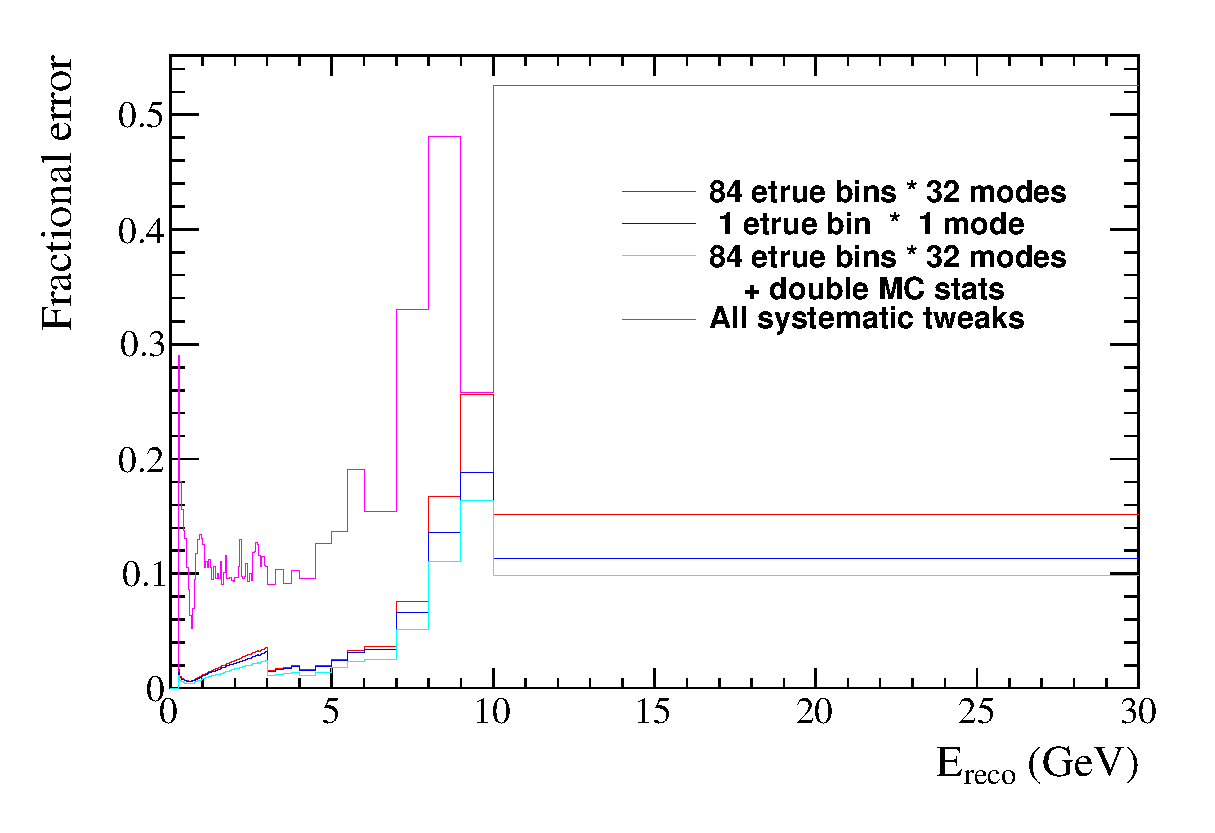
\includegraphics[width=30pc]{./images/mcstaterr_spectrum}
    \caption {
      Fractional error on $N_{SK}$ for three types of statistical error,
      and the total systematic error.
      No oscillations have been applied.
    }
    \label{fig:mc_stat_err_spectrum}
  \end{figure*}

  \begin{figure*}[htb]
    \center
    \begin{minipage}[htb]{0.45\linewidth}
      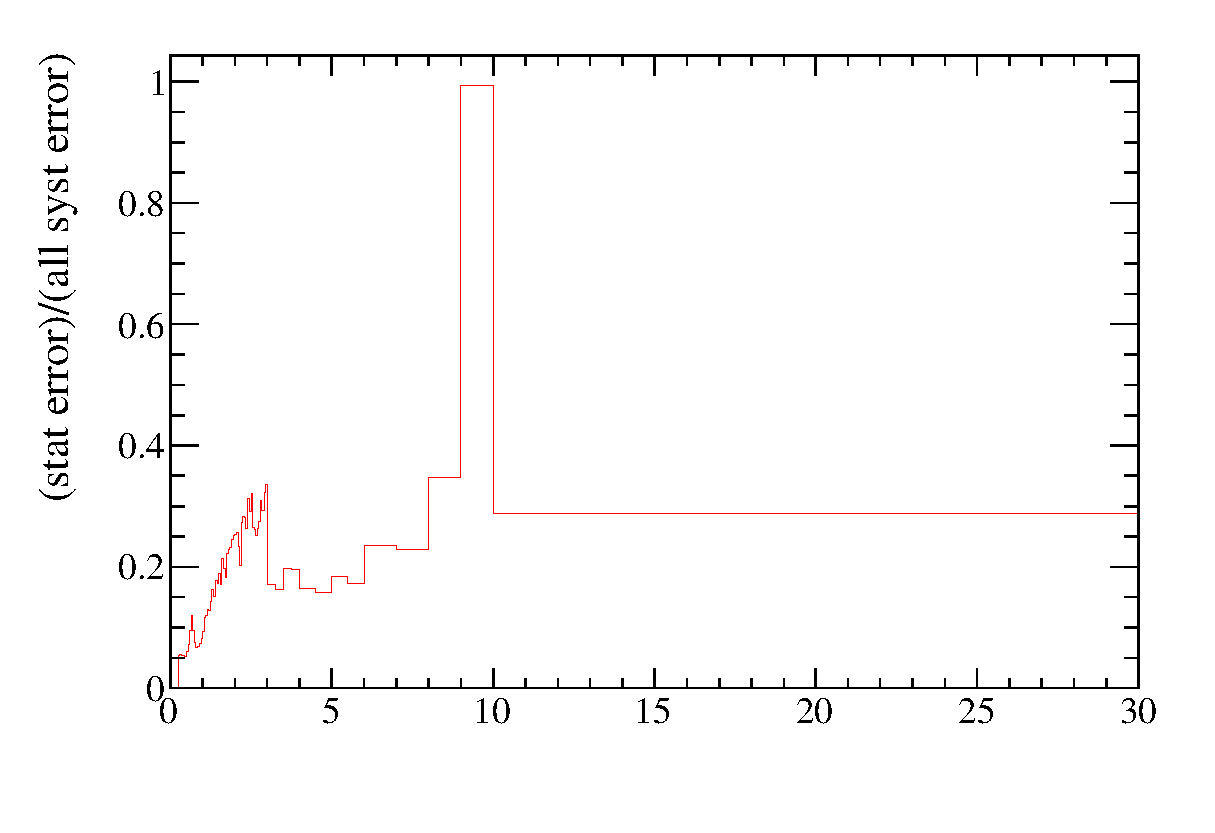
\includegraphics[width=20pc]{./images/mcstaterr_ratio}
      \caption {
        Ratio of MC statistical error to total systematic error.
        No oscillations have been applied.
      }
      \label{fig:mc_stat_err_ratio}    
    \end{minipage}
    \hspace{0.06\linewidth}
    \begin{minipage}[htb]{0.45\linewidth}
      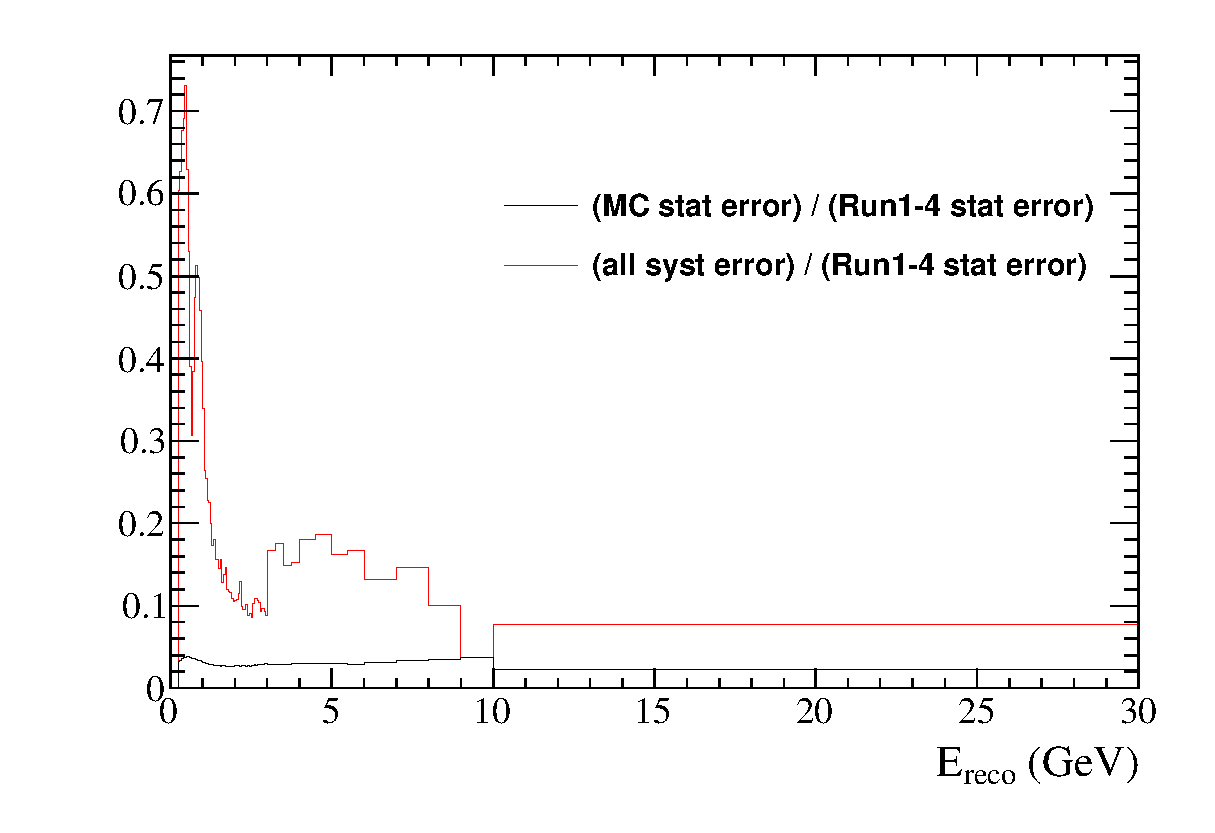
\includegraphics[width=20pc]{./images/mcstaterr_ratio_stat}
      \caption {
        Ratio of MC statistical error and total systematic error
        to Run 1-4 statistical error.
        No oscillations have been applied.
      }
      \label{fig:mc_stat_err_ratio_stat}    
    \end{minipage}
  \end{figure*}

  
  % ........................................................................................................
  \vspace{5 mm}
\item
  {\em
    Figs 59-61:\\
    The 90\% CL horizontal line on these plots seems to be drawn at 2.3, rather than the correct value of 2.7.
    This makes me concerned that you have miscalculated the 90\% 1D confidence intervals in Fig 61.
    Please check this, and state explicitly what $\Delta(\chi^2)$ values were used for the 68\% and 90\% CL limits in Fig 61.
    (Of course I've already stated that I think the FC equivalents are a mandatory addition.)
  }\\
  \\
  You are correct that the incorrect value was used. The plots \& 1D limits have been updated.
  1D limits are calculated using $\Delta \chi^2 =$ 1.00(2.71) for 68\%(90\%).
  2D contours are calculated using $\Delta \chi^2 =$ 2.30(4.61) for 68\%(90\%).
  A footnote has been added to section 7.4 with these values.

  % ........................................................................................................
  \vspace{5 mm}
\item
  {\em
    Given that we haven't had any new data in months, and won't have any, why shouldn't we immediately extend
    this analysis to include ALL Run 4 SK data?  I wouldn't propose to update the ND280 inputs,
    but it really shouldn't be much work to add in the late April-early May 2013 data, should it?
    The beam systematics for that period will almost certainly be identical to that for the rest of Run 4,
    and although the beam inputs to the BANFF fit will have to be adjusted for a slightly different POT weighting,
    this ought to be very fast.  We're going to need to do this anyway, so why not now?
  }\\
  \\
  The decision to use only Run 1-4a data for the first version of
  the 2013 $\nu_\mu$ disappearance analysis was taken by the collaboration.
  The collaboration also agreed to move to the full Run 1-4 dataset for the
  September collaboration meeting.
  Therefore v3 of the note will include all data recorded.

  % ........................................................................................................
  \vspace{5 mm}
\item
  {\em
    Line 435-436:\\
    I find it a little strange that you are throwing random values for $\delta_{CP}$ in the fake data sets
    but are not allowing $\delta_{CP}$ to float in the fit.  It seems a little inconsistent to do one but not the other.
    Can you please justify this choice?
  }\\
  \\
  The constant-$\Delta\chi^2$ normal hierarchy contours for
  $\delta_{CP} = -\pi/2$, 0, $+\pi/2$, $+\pi$
  is shown
  in Fig.\ \ref{fig:constdchisqcontours_changedcp} of this document.
  It can be seen that changing $\delta_{CP}$ has almost no effect on the contour.
  For this reason, and due to the fact that the typical fit time is increased
  by 10\% by including $\delta_{CP}$, it was decided not to fit for it in v1.

  \begin{figure*}[htb]
    \center
    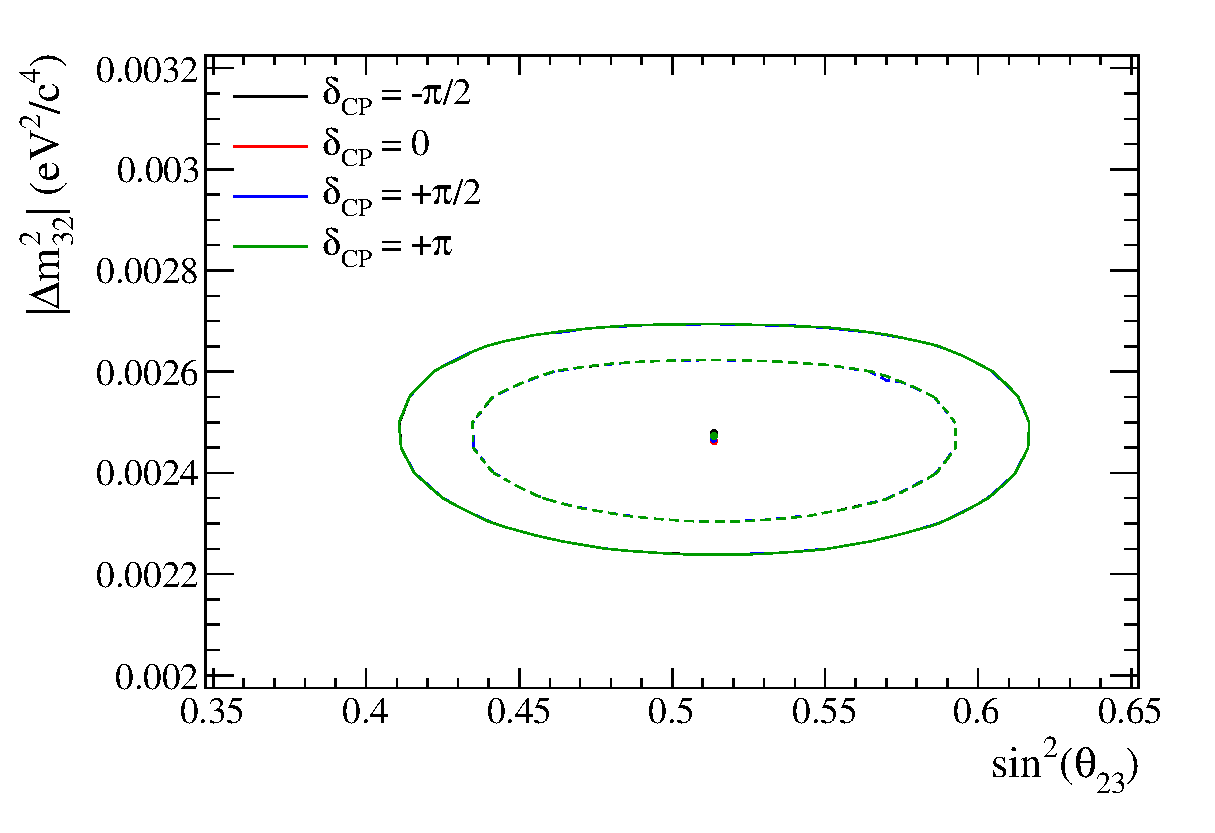
\includegraphics[width=30pc]{./images/contours_run1-4a_nuis3fixdcp_dcp}
    \caption {
      68\% CL and 90\% CL allowed region (including systematics), 
      constructed with the constant-$\Delta\chi^{2}$ method,
      for the fit to the Run 1+2+3+4a dataset,
      for four assumptions of the value of
      $\delta_{CP} = -\pi/2$, 0, $+\pi/2$, $+\pi$.
      The best-fit points are also shown.
      The normal mass hierarchy is assumed.
    }
    \label{fig:constdchisqcontours_changedcp}
  \end{figure*}

  Fitter bias studies have been performed for
  the case where $\delta_{CP}$ is fit for, and compared to the studies
  where $\delta_{CP}$ is set to 0.
  No obvious issues have been found\footnote{
    The pull distribution of $\delta_{CP}$ is irregular,
    due to it having a small effect on the 1-ring $\mu$-like energy spectrum,
    and there being no constraint term, the HESSE assigns
    large errors.
    However this has no effect on the distributions of other parameters.
  }
  to suggest that
  fitting for $\delta_{CP}$ is not possible.
  Therefore in v3 of the note, we will include $\delta_{CP}$ in the fit
  as a free parameter, with no constraint term.

  
  % ........................................................................................................
  \vspace{5 mm}
\item
  {\em
    I have a picky question about the CC1pi normalization (parameter \#21) on p. 13.  The BANFF nominal value (pre-BANFF fit) is 1.15,
    according to TN-166, and you list the fitted value as 1.200 (although TN-166 gives 1.217 instead).  My question
    (besides why 1.200 instead of 1.217) is whether you are interpreting the fitted value as a scale factor relative to 1.15, or
    relative to 1.0?  That is to say, based on the fitted value, do you scale the CC1pi events for this bin by 1.200, or by
    (1.15 x 1.200)?  I don't even know for sure which is right---you may need to ask the BANFF experts.
    Really I just want some reassurance that everyone is interpreting this scale factor consistently.  All(?) of the
    other scale factor parameters have nominal values of 1.0, so this question may not arise for them.
  }\\
  \\
  The discrepancy in values is due to inconsistent BANFF fit versions described in the notes.
  We treat it as (1.00 x 1.200).
  I have confirmed with Mark Hartz that is correct.
  
  % ........................................................................................................
  \vspace{5 mm}
\item
  {\em
    p. 13:\\
    please state explicit the form of the constraint term, if any, for $f_{SF; t, r}$.  I couldn't find it in TN-141 either.
    I'm guessing that you have no constraint term other than bounding the parameter to the region [0,1]?  Please confirm.
  }\\
  \\
  For v1 of the note, there is a constraint term, and it has the same form as any other systematic terms. Namely,
  \begin{equation}
    \frac{f_{bf} - f_{nom}}{\sigma_{nom}^2},
  \end{equation}
  since it is not correlated with any other systematic.
  The boundary of [0,1] is also applied, meaning the penalty runs from [0,1].

  After thinking about this,
  for v3 of the note, we will have no constraint term.
  This is because we throw the parameter uniformly in the range [0,1]
  when generating toy experiments, and so having a constraint which favours
  $f_{SF; t, r} = 0$ is unnatural.

  % TN113v1.2
  % 471 The uncertainty is scaled such that the 1σ uncertainty is set to be the difference
  % 472 between SF and FG, 0 is no difference, and all other values are linearly extrapolated
  % 473 or interpolated (e.g. 2σ is twice the SF/FG difference). While this is nonphysical,
  % 474 it was not obvious how to treat a discrete (on/off) parameter in the 2012a fits. In
  % 475 addition, a smooth parametrization allows us to see where the fit moves this nuisance
  % 476 parameter according to agreement with data. An inherent limitation to the current
  % 477 parametrization is that the SF prediction populates regions of true p − θ where FG
  % 478 does not, and this cannot be treated with reweighting. An example of this can be
  % 479 seen in Figure 64 which shows NuWro SF populates p < 0.3 GeV/c and cos(θ) > 0.3,
  % 480 not present in either FG model; note that the cross section in this region is much
  % 481 smaller than in the primary region.

  % ........................................................................................................
  \vspace{5 mm}
\item
  {\em
    Pull distribution figures:\\
    why is the width of the pull distribution for $f^{SK}_{E;r}$ usually 1.15 instead of the expected 1.0. 
  }\\
  \\
  This is to do with the fact that the effect of the $f^{SK}_{E;r}$ systematic on
  the number of events in a bin is not a smooth function of $f^{SK}_{E;r}$;
  it is continuous, but it's differential is not.
  This is due to the systematic being dependant on the number of events in neighbouring bins,
  and so there is a discontinuity in the differential when moving from positive to negative
  values of $f^{SK}_{E;r}$, and also at large values of $f^{SK}_{E;r}$ when next-to-neighbouring
  bins come into effect.
  Therefore HESSE has a problem evaluating errors for this parameter.
  If we instead use MINOS errors, the distribution is as expected, as shown
  in Fig.\ \ref{fig:skescale_pull} of this document.
  The residual distribution exhibits the correct behaviour.

  \begin{figure*}[htb]
    \center
    \includegraphics[width=25pc]{{./images/fixdcpminos_sys_0.37_pull_1_escale}.eps}
    \caption {
      Pull distribution for $f^{SK}_{E;r}$,
      computed from 5.1k toy MC experiments at 6.3933×1020 POT,
      generated at
      at $\sin^2\theta_{23} = 0.65$ and $|\Delta m^2 | = 2.4\times10^{−3}$ eV$^2$/c$^4$, including
      statistical fluctuations and with randomized systematic parameters.
      MINOS errors are used.
    }
    \label{fig:skescale_pull}
  \end{figure*}

  % ........................................................................................................
  \vspace{5 mm}
\item
  {\em
    Fig 17:\\
    I understand the three peaks in Figs 15 and 19 (true point, mirror point, and point of maximum disappearance).
    But I don't understand Fig 17, where there are also three humps (although two are quite small), even
    though the best-fit point should be the same as the point of maximual disappearance.  Please comment.
  }\\
  \\
  This is still under study.

  % ........................................................................................................
  \vspace{5 mm}
\item
  {\em
    Line 371:\\
    Shouldn't you be citing Ref [22] rather than Ref [15], and referring to CC0pi, CC1pi, and CCother samples rather
    than CCQE and CCnQE?  Doesn't this analysis use the 2013 BANFFv2 fit results and not 2012 BANFF fits?
  }\\
  \\
  Correct, this has been updated.

  % ........................................................................................................
  \vspace{5 mm}
\item
  {\em
    Line 442:\\
    point of clarification: do these 7 parameters include 1 energy scale and 6 detector/FSI efficiency parameters?
  }\\
  \\
  Yes.
  The bullet point list \& Tab.\ 1 headings have been updated.
  
  % ........................................................................................................
  \vspace{5 mm}
\item
  {\em
    Top of p. 13:\\
    again you are citing Ref [15] (old BANFF) rather than [22] (new 2013 BANFF).  Why?  
  }\\
  \\
  This has been corrected.

  % ........................................................................................................
  \vspace{5 mm}
\item
  {\em
    Table 3:\\
    Of course I can't imagine it mattering, but why did you use $\Delta m^2_{21}=7.5\times 10^{-5}$
    instead of the PDG2012 value of $7.58\times 10^{-5}$?
  }\\
  \\
  When choosing values of oscillation parameters, we have used the particle
  listings section of reference 28.

  The value $7.58 \times 10^{-5}$ is shown on p193,
  which is in the review of neutrino mixing, and is the result of a
  3-flavour fit, incorporating neutrino oscillation data (but not Daya Bay \& RENO).
  
  The value $7.50 \times 10^{-5}$ is shown on p642,
  which is the particle listings, and is the result of a 3-flavour fit
  on KAMLAND + solar data.

  % ........................................................................................................
  \vspace{5 mm}
\item
  {\em
    Table 7:\\
    are the values in this table in percent?  If so, please state that in the caption.
  }\\
  \\
  Yes, this has been corrected.

  % ........................................................................................................
  \vspace{5 mm}
\item
  {\em
    Pull distribution figures:\\
    several figures have fitted means of 1.0 and sigmas of 0.  This can't be right.  I'm guessing these are failed fits---can you please fix them?
  }\\
  \\
  There are 4 fits that had a fitted sigma of 1, with an error on this value of 0.0 according to the plots.
  All 4 fits were fine (no failed fits) it was just the way ROOT was reporting the error in the stat box
  (it appears that ROOT rounds \& kills trailing zeros in the parameter value, then quotes errors to this significance).
  The plots have been updated with more significant figures in the fit stat box.
  
  % ........................................................................................................
  \vspace{5 mm}
\item
  {\em
    Fig 49, and many other figures:\\
    The legends printed on this plot, and those like them, are too small to be acceptable for publication in Phys. Rev.
    If these are to become official plots, please remake them with larger, more legible legends.
  }\\
  \\
  We have increased the legend size of some plots in v2 of the note,
  but have not done them all, since for some plots this was the only comment.
  When we release v3, with the results from the fixed SuperK detector error matrix,
  we will update the legends in the rest of the plots.
  
  % ........................................................................................................
  \vspace{5 mm}
\item
  {\em
    Figs 55 \& 56 captions:\\
    You mean Run 1+2+3+4a, not Run 1+2+3
  }\\
  \\
  This has been corrected.

  % ........................................................................................................
  \vspace{5 mm}
\item
  {\em
    Line 734:\\
    How was the marginalization by octant done?  Did you average the contours, or did you simply take the larger of the two contours?
  }\\
  \\
  From D. Karlen's comments on the Run 1-3 PRL, we realise that the wrong terminology was originally used.
  The method is, in fact, profiling.
  
  For every point in $\sin^2(2\theta_{23})$ there are 2 points in $\sin^2\theta_{23}$ for which the $\Delta \chi^2$
  and $\Delta\chi^2_{crit}$ are known.
  The $\sin^2\theta_{23}$ point with the lowest $\Delta\chi^2 - \Delta\chi^2_{crit}$ is chosen.
  The $\sin^2(2\theta_{23})$ contour created will be similar to the second octant contour
  if an octant preference is made.
  Fig.\ \ref{fig:contours_sinsq2theta_method} of this document shows that in this case, the
  profiled and second octant contours are identical.  

  \begin{figure*}[htb]
    \center
    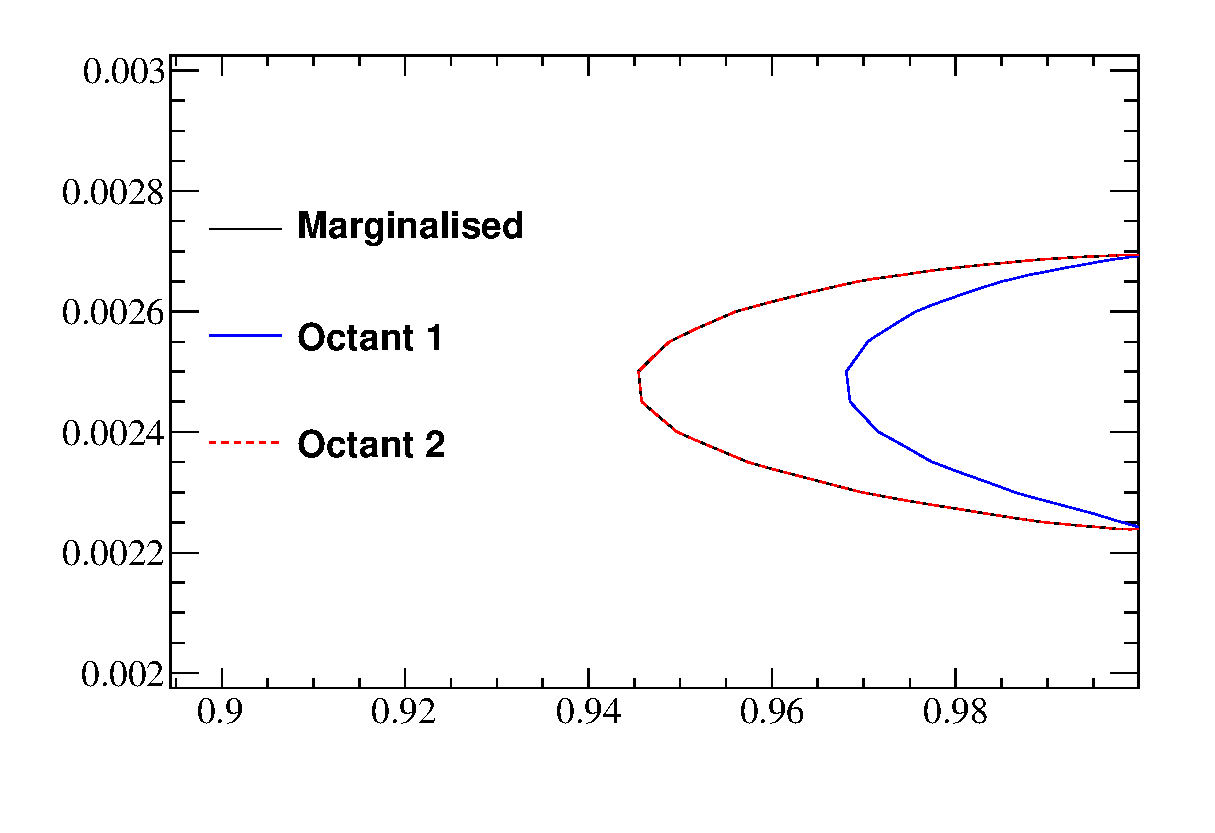
\includegraphics[width=30pc]{./images/sinsq2theta_conversion}
    \caption {
      68\% CL and 90\% CL allowed region (including systematics), 
      constructed with the constant-$\Delta\chi^{2}$ method,
      for the fit to the Run 1+2+3+4a dataset.
      The contour is converted into $\sin^2(2\theta_{23})$ in three ways:
      profiling over octant;
      assuming the first octant;
      assuming the second octant.
      The normal mass hierarchy is assumed.
    }
    \label{fig:contours_sinsq2theta_method}
  \end{figure*}
  


  % ........................................................................................................

\end{enumerate}

